\section{Informatiesystemen}

\subsection{Het belang van informatie}

\bi
\itf 
\itf 
\itf 
\itf 
\itf 
\itf 
\itf 
\itf 
\itf 
\itf 
\itf 
\itf 
\itf 
\itf 
\itf 
\itf 
\itf 
\itf 
\itf 
\itf 
\itf 
\itf 
\itf 
\itf 
\ei


\subsection{Een informatiesysteem}

\subsubsection{What is an \Gls{informationsystem} ?}

\textcolor{red}{\Gls{system}} = collection of interacting components, which are arranged according to a certain plan in order to achieve a particular goal

Systeem = een verzameling op elkaar inwerkende componenten, die volgens een bepaald plan geordend zijn, teneinde een bepaald doel te bereiken.

\textcolor{red}{\Gls{informationsystem}} = system that is responsible for collecting, managing, storing and processing of data and for providing information that is of value in forming judgments and to perform activities in the organization


\subsection{Characteristics of a System}

\begin{figure}[htp]
    \centering
            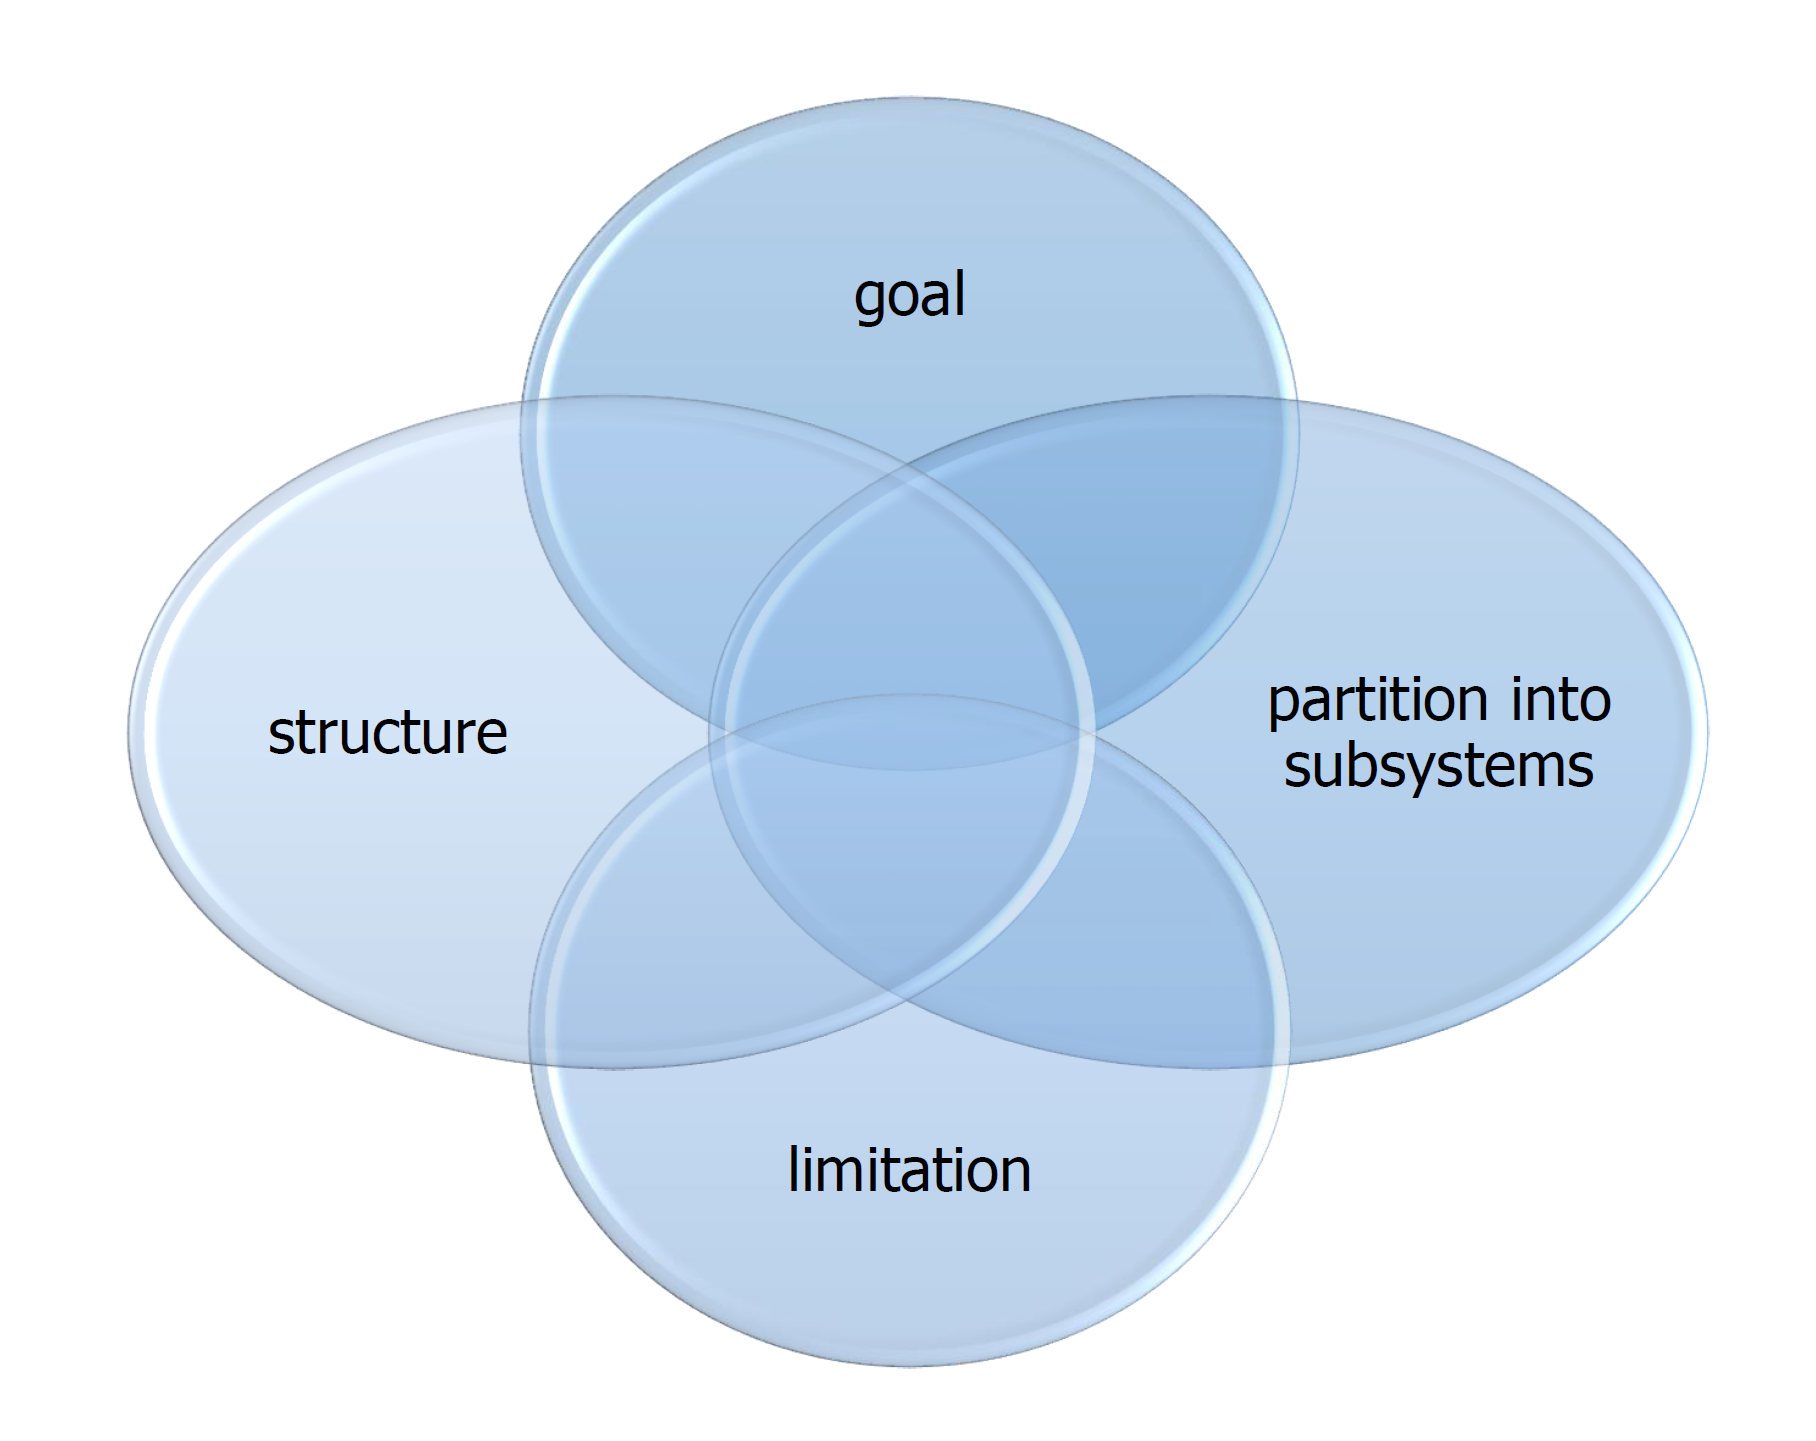
\includegraphics[width=4in]{img/osa1.PNG}
        \caption{Characteristics of a System}
    \label{fig:Characteristics of a System}
\end{figure}

\be
\itf 
\itf 
\itf 
\itf 
\itf 
\itf 
\itf 
\itf 
\itf 
\itf 
\itf 
\itf 
\itf 
\itf 
\itf 
\itf 
\itf 
\itf 
\itf 
\itf 
\itf 
\itf 
\itf 
\itf 
\ee


\subsubsection{Definitie}

\subsubsection{InformatieSysteem}

\subsubsection{Kenmerken}

\subsubsection{Eisen voor een goed systeem}

\subsubsection{Modellen}

%3.
\subsection{De evolutie in systeemanalyse}

\subsubsection{}

\subsection{}

\subsection{}

\subsection{}